本章分别分析源码与二进制程序识别、源码参考库补充、固件镜像识别及前端应用验证的实验结果。算法识别以文件--算法组合为统计单位，分别报告正确检出（TP）、误报（FP）和漏报（FN）；同一文件中支持相同算法的多条证据合并计数。固件镜像实验考察五类终端的组件提取与算法实现识别，前端实验则以电力边缘网关检验结果展示、证据定位和报告导出的一致性。

\section{十三种算法识别结果}
\label{sec:algorithm-suite-results}

\subsection{总体识别结果与逐算法分析}

本组实验评价工具对已参与开发的已知实现的识别表现。本组共检测 1071 份文件，以人工审核的“文件--算法”组合为统计单位，共有 747 项应检出的算法实现。同一文件包含多种算法时分别计数，同一算法的多条证据不重复计数。工具正确检出其中 726 项，漏报 21 项，未产生评分范围内的误报。总体召回率为 97.19\%，精确率为 100.00\%，漏报率为 2.81\%。按第三章确定的已审核标签范围，另有 11206 个真阴性标签，准确率为 99.82\%。由于阴性标签数量较多，以下主要结合召回率和精确率分析识别效果。

表~\ref{tab:algorithm-suite-algorithms} 给出十三种算法的识别结果。AES、ECDSA、ECDH、MD5 和 SM4 未出现漏报，其余算法的漏报率为 1.56\%--7.89\%，各算法合并载体后的漏报率均低于 10\%。SHA-256 的漏报率最高，6 个漏报占全部漏报的 28.57\%；SHA-256、SM3 和 SM2 合计占 13 个，构成该集合中覆盖不足的主要部分。

\begin{table}[!htbp]\centering\small
\caption{十三种算法在已知实现集合上的识别结果}
\label{tab:algorithm-suite-algorithms}
\begin{tabularx}{\linewidth}{@{}Xrlrr@{}}\toprule
算法 & 应检出数 & TP/FP/FN & 召回率 & 漏报率\\\midrule
AES & 66 & 66/0/0 & 100.00\% & 0.00\%\\
DES & 63 & 61/0/2 & 96.83\% & 3.17\%\\
RC4 & 55 & 53/0/2 & 96.36\% & 3.64\%\\
ChaCha20 & 64 & 63/0/1 & 98.44\% & 1.56\%\\
RSA & 36 & 35/0/1 & 97.22\% & 2.78\%\\
ECDSA & 32 & 32/0/0 & 100.00\% & 0.00\%\\
ECDH & 47 & 47/0/0 & 100.00\% & 0.00\%\\
MD5 & 53 & 53/0/0 & 100.00\% & 0.00\%\\
SHA-1 & 56 & 54/0/2 & 96.43\% & 3.57\%\\
SHA-256 & 76 & 70/0/6 & 92.11\% & 7.89\%\\
SM2 & 66 & 63/0/3 & 95.45\% & 4.55\%\\
SM3 & 70 & 66/0/4 & 94.29\% & 5.71\%\\
SM4 & 63 & 63/0/0 & 100.00\% & 0.00\%\\\bottomrule
\end{tabularx}
\end{table}

图~\ref{fig:algorithm-suite-algorithms} 同时给出各算法的正标签数量和漏报率。各分组包含 32--76 个正标签，百分比差异应结合分母理解。上述结果表明，工具在已收录实现及相应构建条件下具有较高覆盖，现有误差主要表现为正标签未检出。

% 配图依据：full-suite-rescan/scan/summary.json；由 algorithm-result-figure/plot.py 重绘并核对逐文件计数。
% 图中 10% 虚线为预设漏报率参考线；保留开发范围说明。
\begin{figure}[!htbp]\centering
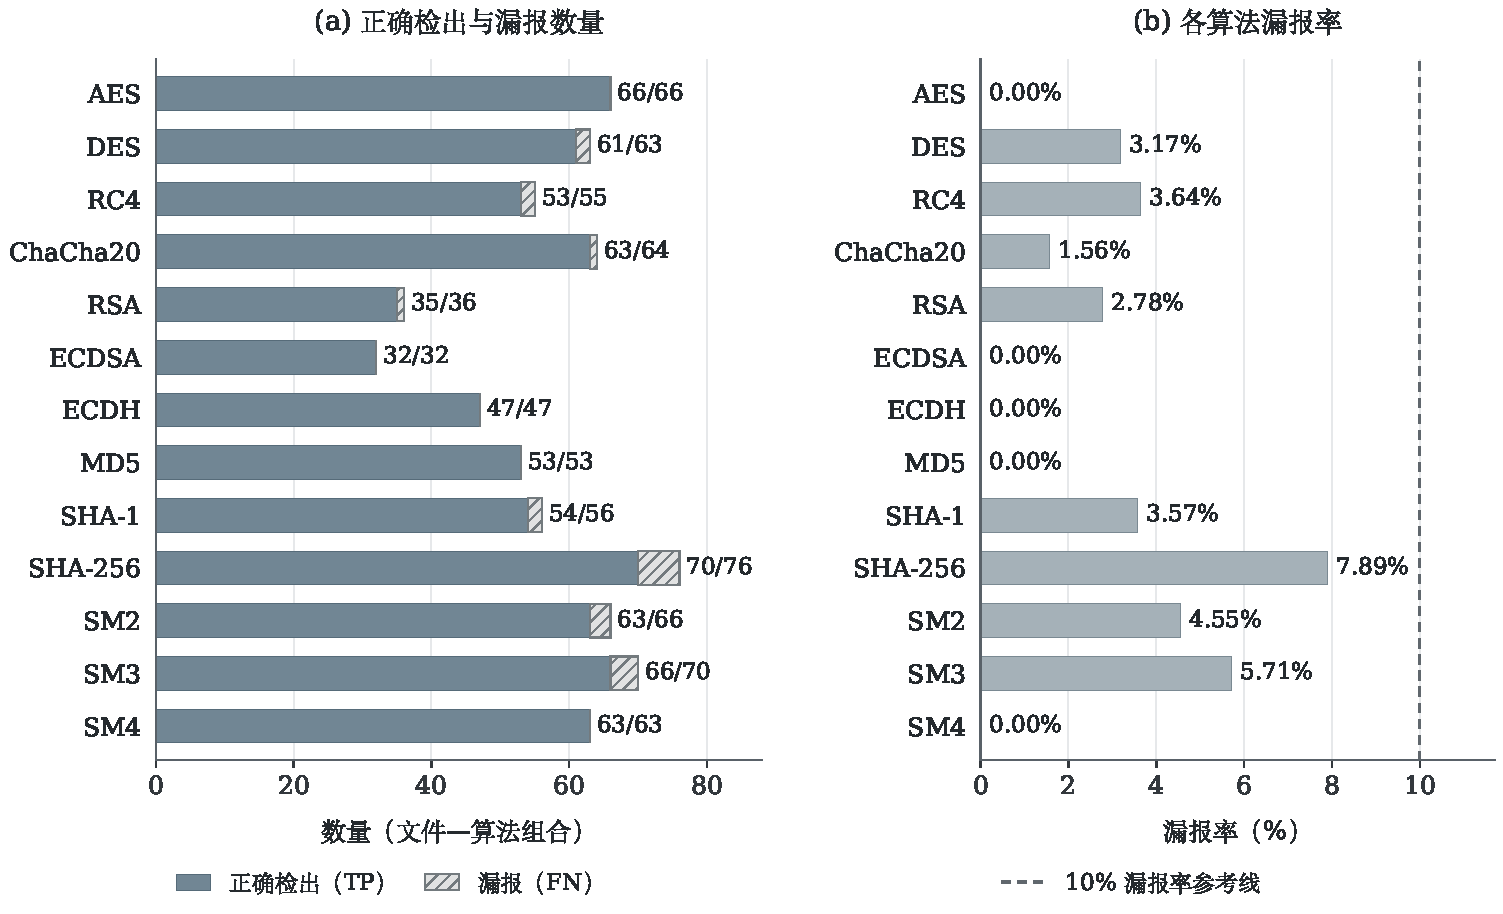
\includegraphics[width=\linewidth]{16-thirteen-algorithms.pdf}
\caption{十三种算法的正确检出、漏报数量及漏报率。左图标注为正确检出数/应检出数，斜线填充表示漏报；右图虚线表示 10\% 漏报率参考线。}
\label{fig:algorithm-suite-algorithms}
\end{figure}

\subsection{源码与二进制程序的识别结果}

表~\ref{tab:algorithm-suite-kinds} 列出源码与两种架构二进制程序的识别结果。154 份源码的召回率为 99.05\%，527 份 x86-64 二进制程序与 390 份 ARM64 二进制程序分别为 97.51\% 和 96.09\%。源码组漏报 1 项，二进制程序组共漏报 20 项。源码分析利用词法、定义及直接依赖信息，二进制程序分析则依据编译后可恢复的字节特征与运算关系。由于三组材料的实现来源和算法构成不同，不能仅据上述差异判断载体或架构对识别效果的影响。本组 1071 份文件不含固件镜像，固件采用独立的镜像集合评价提取与识别结果。

\begin{table}[H]\centering\small
\caption{源码与不同架构二进制程序的识别结果}
\label{tab:algorithm-suite-kinds}
\begin{tabularx}{\linewidth}{@{}Xrrlrr@{}}\toprule
检测对象 & 文件 & 应检出数 & TP/FP/FN & 召回率 & 漏报率\\\midrule
源码 & 154 & 105 & 104/0/1 & 99.05\% & 0.95\%\\
x86-64 二进制程序 & 527 & 361 & 352/0/9 & 97.51\% & 2.49\%\\
ARM64 二进制程序 & 390 & 281 & 270/0/11 & 96.09\% & 3.91\%\\\bottomrule
\end{tabularx}
\end{table}

% 配图依据：full-suite-rescan/scan/summary.json；由 plot_carriers.py 重算39个单元格并核对算法、载体两方向合计。
% 保留 ChaCha20 源码子组 1/8，不将标注边界通过重命名或删样本消除。
\begin{figure}[H]\centering
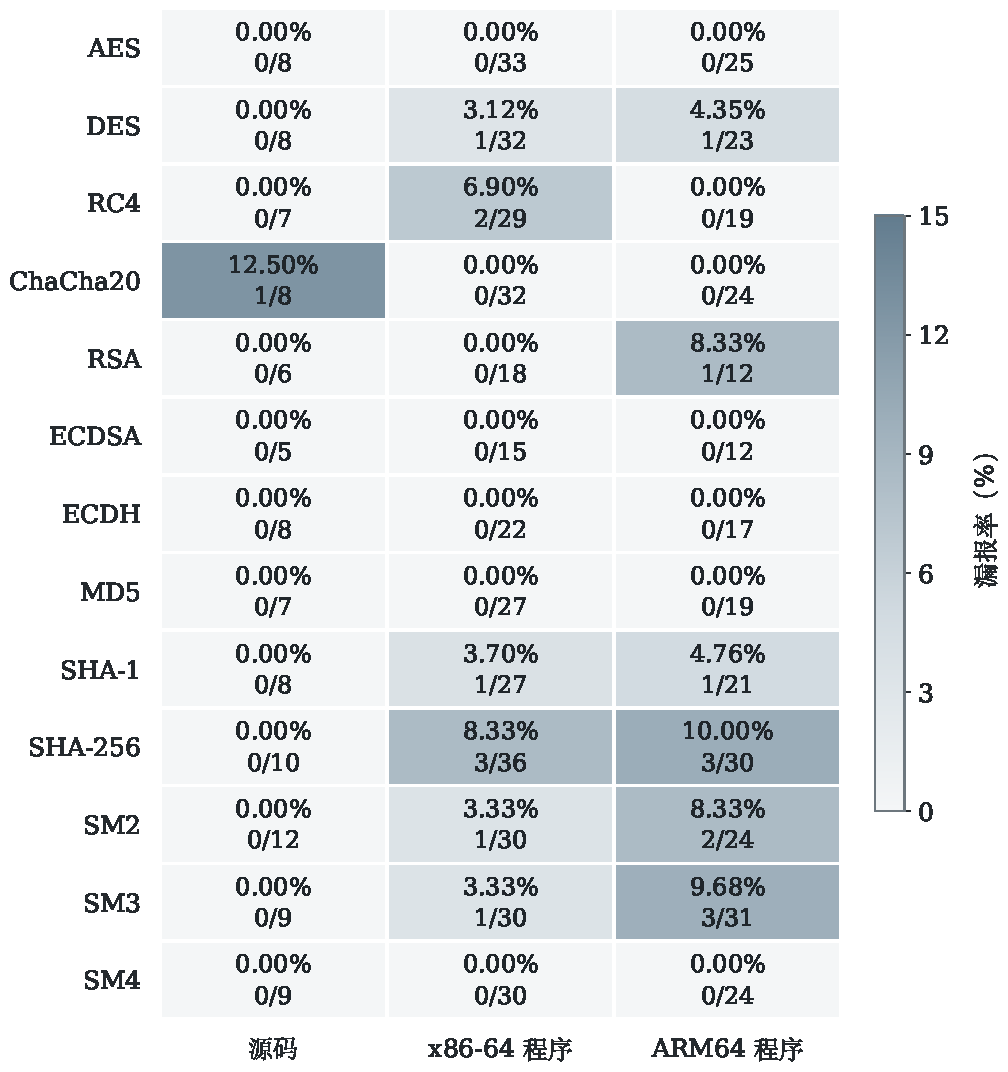
\includegraphics[width=.9\linewidth,height=.72\textheight,keepaspectratio]{17-thirteen-carriers.pdf}
\caption{十三种算法在源码、x86-64 和 ARM64 分组中的漏报分布。单元格上行为漏报率，下行为漏报数/应检出数。}
\label{fig:algorithm-suite-carriers}
\end{figure}

图~\ref{fig:algorithm-suite-carriers} 进一步展示算法与载体交叉分组的漏报情况。源码组中十二种算法均无漏报，ChaCha20 保留 1/8 的原正标签未检出。对该文件的复核发现，其循环实际执行八轮变换，属于 ChaCha8，与原 ChaCha20 标注不一致。为保持固定清单的评分口径，该项仍按原标签计入漏报，并单独说明变体差异。因此，算法总体漏报率低于 10\% 并不意味着所有载体子组都达到同一水平。

全部 1071 份文件均完成分析，未出现部分完成或失败。在 16 进程并发条件下，整批扫描耗时 498.03 秒。该耗时为单次运行记录，仅用于说明本组实验的处理成本。

\section{源码参考库消融实验结果}
\label{sec:expanded-source-results}

\subsection{参考补充对总体识别结果的影响}

表~\ref{tab:expanded-source-ablation} 给出 363 份源码、318 个实现正标签上的配对结果。两组固定检测器代码、输入及可见上下文，仅将源码参考库由 149 条扩充至 226 条。补充前正确检出 225 个正标签，漏报 93 个；补充后正确检出 306 个，漏报降至 12 个。召回率由 70.75\% 提高到 96.23\%，精确率由 99.56\% 变为 99.67\%。

\begin{table}[H]\centering\small
\caption{参考库补充前后的源码识别结果}
\label{tab:expanded-source-ablation}
\begin{tabularx}{\linewidth}{@{}Xrlrrr@{}}\toprule
参考库 & 记录数 & TP/FP/FN & 召回率 & 精确率 & 漏报率\\\midrule
原参考库 & 149 & 225/1/93 & 70.75\% & 99.56\% & 29.25\%\\
扩充参考库 & 226 & 306/1/12 & 96.23\% & 99.67\% & 3.77\%\\\bottomrule
\end{tabularx}
\end{table}

逐文件比较表明，补充参考记录增加了 81 个正确标签，未丢失原有正确检出，误报数量保持为 1，召回率提高 25.47 个百分点。新增 77 条记录中存在多算法模块，因此记录增量与标签增量并非一一对应。该配对结果反映固定代码条件下已知内容覆盖的变化，两组均保留其他识别通道。

两组均有 362 份源码正常完成、1 份部分完成，未出现失败。部分完成文件中的 ECDH 已被参考记录识别，但两个函数的结构分析达到节点预算上限，故其处理状态仍保留为部分完成。补充前后批次耗时分别为 70.72 秒和 72.14 秒；测量期间存在并发任务，仅据此记录处理规模，不将二者之差解释为参考库扩充的运行代价。

\subsection{来源分组结果与剩余误差}

表~\ref{tab:expanded-source-cohorts} 将参考补充及标签变化按材料来源分组。新增 77 条参考全部取自该源码集合，其中 59 条来自 110 份历史验证来源源码，占该子组文件数的 53.64\%。原参考库已有 120 条记录与待测源码内容重叠，扩充后增至 197 条。因此，该实验评价已观察材料上的版本覆盖，“历史验证来源”仅表示材料原始出处。

\begin{table}[H]\centering\small
\caption{不同来源源码的参考补充与识别结果}
\label{tab:expanded-source-cohorts}
\begin{tabularx}{\linewidth}{@{}Xrrrll@{}}\toprule
来源 & 文件 & 应检出数 & 新增参考 & 补充前 & 补充后\\\midrule
原固定源码 & 154 & 103 & 0 & 103/0/0 & 103/0/0\\
其他历史开发源码 & 71 & 72 & 1 & 70/0/2 & 71/0/1\\
历史验证来源源码 & 110 & 115 & 59 & 41/0/74 & 104/0/11\\
新审核模块 & 28 & 28 & 17 & 11/1/17 & 28/1/0\\
合计 & 363 & 318 & 77 & 225/1/93 & 306/1/12\\\bottomrule
\end{tabularx}
\par\smallskip\raggedright\footnotesize 注：补充前、补充后两列均按 TP/FP/FN 表示。
\end{table}

历史验证来源子组增加 63 个正确标签，召回率由 35.65\% 提高到 90.43\%，误报仍为零，是总体增益的主要来源。由于其中 59 份源码已参与参考库构建，该结果表明相应版本纳入参考后的覆盖改善，不再具有独立测试的含义。新审核模块增加 17 个正确标签，其他历史开发源码增加 1 个，原固定源码的预测保持不变。

本组对原固定源码采用经核查的 103 个正标签：一份 ChaCha8 和一份仅含四分之一轮的源码均保留为输入，但不赋予完整 ChaCha20 标签。该组的 103/0/0 与上一节的 104/0/1 因评分范围不同而形成，实际预测一致，不属于新增检出。

表~\ref{tab:expanded-source-algorithms} 列出扩充参考库后的逐算法结果。各算法包含 20--55 个正标签，漏报率均不超过 10\%。DES、RC4、ECDSA、ECDH 和 MD5 无漏报；SHA-1 的漏报率最高，为 9.09\%。ECDH 同时出现 1 项误报，说明正标签覆盖与算法身份判定仍需分别考察。

\begin{table}[H]\centering\small
\caption{扩充参考库后的逐算法源码识别结果}
\label{tab:expanded-source-algorithms}
\begin{tabularx}{\linewidth}{@{}Xrlrr@{}}\toprule
算法 & 应检出数 & TP/FP/FN & 召回率 & 漏报率\\\midrule
AES & 55 & 53/0/2 & 96.36\% & 3.64\%\\
DES & 20 & 20/0/0 & 100.00\% & 0.00\%\\
RC4 & 20 & 20/0/0 & 100.00\% & 0.00\%\\
ChaCha20 & 20 & 19/0/1 & 95.00\% & 5.00\%\\
RSA & 26 & 24/0/2 & 92.31\% & 7.69\%\\
ECDSA & 21 & 21/0/0 & 100.00\% & 0.00\%\\
ECDH & 21 & 21/1/0 & 100.00\% & 0.00\%\\
MD5 & 21 & 21/0/0 & 100.00\% & 0.00\%\\
SHA-1 & 22 & 20/0/2 & 90.91\% & 9.09\%\\
SHA-256 & 31 & 29/0/2 & 93.55\% & 6.45\%\\
SM2 & 21 & 20/0/1 & 95.24\% & 4.76\%\\
SM3 & 20 & 19/0/1 & 95.00\% & 5.00\%\\
SM4 & 20 & 19/0/1 & 95.00\% & 5.00\%\\\bottomrule
\end{tabularx}
\end{table}

12 个漏报中有 11 个位于历史验证来源子组，另一个位于其他历史开发源码。漏报文件涉及实现主体委托、可见上下文不足和硬件专用表示等情况。唯一误报位于 LibreSSL 的 SM2 加解密模块，共享椭圆曲线点运算额外触发 ECDH 标签，反映出公共数学结构与具体协议用途之间的区分仍不充分。

\section{固件镜像识别结果}
\label{sec:firmware-results}

\subsection{镜像提取与终端覆盖}

本组以五类终端的 10 份自制 SquashFS 镜像为检测对象，每类分别提供 x86-64 和 ARM64 版本。扫描器直接接收原始镜像，提取内部文件后执行静态分析，镜像内部不包含源码。全部镜像均完成提取与扫描，共恢复 650 个文件，其中二进制文件 540 个。恢复文件的路径和内容摘要与独立交付清单逐项一致，未发现组件遗漏或内容变化。

每份镜像含 65 个文件，其中 54 个为二进制文件。除原业务程序及其密码库外，另有十三种算法的 13 个共享库和 39 个静态链接程序。三个程序变体分别处理原始输入、带长度字段的记录及带终端任务标识的记录，所需算法代码均实际链接于文件内部。十份镜像共有 530 个文件包含密码实现，其他文件仅保留运行所需配置、输入、说明和许可。共享库保留导出接口，离线程序保留普通符号表，故本组包含不同符号条件，不能统一解释为去符号识别成绩。

五类 x86-64 镜像中的 65 个新增共享库、195 个新增程序均通过功能检查，5 个原业务程序也通过预期输出核对。九种对称或摘要算法的已知答案检查通过，RSA、ECDSA 和 SM2 完成正常签名验签与篡改拒绝检查，ECDH 双方所得共享秘密一致。新增程序可独立处理本地输入，但未自动接入原业务服务，不将组件存在等同于业务已启用全部算法。ARM64 仅完成构建、提取与静态扫描。

\begin{table}[H]\centering\small
\caption{五类终端固件的提取与实现识别结果}
\label{tab:terminal-coverage-results}
\begin{tabularx}{\linewidth}{@{}Xrrrl@{}}\toprule
终端软件类型 & 镜像 & 提取文件 & 二进制文件 & TP/FP/FN\\\midrule
智能电能表 & 2 & 130 & 108 & 131/0/9\\
用电信息采集集中器 & 2 & 130 & 108 & 131/0/9\\
配电自动化终端（FTU） & 2 & 130 & 108 & 131/0/9\\
继电保护装置（IED） & 2 & 130 & 108 & 131/1/9\\
电力边缘网关 & 2 & 130 & 108 & 133/0/9\\
合计 & 10 & 650 & 540 & 657/1/45\\\bottomrule
\end{tabularx}
\end{table}

\subsection{算法识别与误差分析}

算法评价以组件的“文件--算法”组合为单位，对清单声明的全部 540 个二进制文件，在十三种目标算法范围内评分。RSA、ECDSA 和 ECDH 组件中的 SHA-256，以及 SM2 组件中的 SM3，均按实际链接内容计入真值。同一算法在多个文件中出现分别计数，同一文件的重复证据合并。文本、配置及许可文件不参与实现评分，本组结果也不与前述 1071 份文件合并计算。

共计 702 项应检出的算法实现，正确检出 657 项，误报 1 项，漏报 45 项。总体召回率为 93.59\%，精确率为 99.85\%，漏报率为 6.41\%。表~\ref{tab:firmware-algorithm-results} 给出逐算法结果，十三种算法均在本组获得正确检出，但不同算法及架构的覆盖并不相同。

\begin{table}[H]\centering\small
\caption{固件镜像内部组件的算法识别结果}
\label{tab:firmware-algorithm-results}
\begin{tabularx}{\linewidth}{@{}Xrlrr@{}}\toprule
算法 & 应检出数 & TP/FP/FN & 召回率 & 精确率\\\midrule
AES & 44 & 44/0/0 & 100.00\% & 100.00\%\\
DES & 40 & 40/0/0 & 100.00\% & 100.00\%\\
SM4 & 44 & 24/0/20 & 54.55\% & 100.00\%\\
RC4 & 40 & 15/0/25 & 37.50\% & 100.00\%\\
ChaCha20 & 40 & 40/0/0 & 100.00\% & 100.00\%\\
MD5 & 42 & 42/0/0 & 100.00\% & 100.00\%\\
SHA-1 & 42 & 42/1/0 & 100.00\% & 97.67\%\\
SHA-256 & 170 & 170/0/0 & 100.00\% & 100.00\%\\
SM3 & 80 & 80/0/0 & 100.00\% & 100.00\%\\
RSA & 40 & 40/0/0 & 100.00\% & 100.00\%\\
ECDSA & 40 & 40/0/0 & 100.00\% & 100.00\%\\
ECDH & 40 & 40/0/0 & 100.00\% & 100.00\%\\
SM2 & 40 & 40/0/0 & 100.00\% & 100.00\%\\
合计 & 702 & 657/1/45 & 93.59\% & 99.85\%\\\bottomrule
\end{tabularx}
\end{table}

按架构汇总，x86-64 组件的 TP/FP/FN 为 346/1/5，ARM64 为 311/0/40。漏报集中于新增 RC4 和 ARM64 SM4 组件：五份 x86-64 RC4 共享库未确认实现，每份 ARM64 镜像中新增的 RC4 共享库及三个程序、SM4 共享库及三个程序均未确认。相关代码已经通过原生功能检查或构建清单审核，缺少识别标签反映当前检测覆盖不足，不能据此否定文件中存在相应实现。唯一误报仍位于 x86-64 继电保护装置的原密码库，实际包含 MD5 和 SHA-256，却额外报告 SHA-1。

算法证据可通过镜像摘要、内部路径及组件摘要回到交付文件。上述结果验证了较多密码组件共存时的提取、识别与定位流程，但多个终端、程序变体及架构复用上游实现，新增文件数量不代表独立实现来源的增加。镜像也不包含完整设备启动环境，因此不能据此推断真实厂商固件或未收录实现的识别水平。

\section{前端应用实验结果}
\label{sec:frontend-results}

本节选取上述电力边缘网关的 x86-64 镜像，验证工作台从任务创建到报告导出的应用流程。该样例复用固件实验中的输入，页面任务单独执行，其识别结果不作为新增独立样本重复计数。

\subsection{网关检测结果与证据定位}

网关镜像大小为 4132864 字节，包含 54 个二进制文件及必要配置、输入与许可材料。工作台独立创建任务后恢复 65 个文件，所有组件均正常完成。服务端端到端耗时为 136.54 秒，包含交付核验、解包、扫描与结果写出，不含浏览器传输和人工查看时间。该数值为本次应用验证的单轮记录。

结果形成 70 条已识别资产记录，涉及全部十三种算法，其中 16 条标为“量子迁移关注”，15 条标为“遗留算法关注”。资产按组件、算法及证据类别归并，多条命中不重复增加记录。一份组件可含多个算法，因此资产记录数与二进制文件数分别统计。图~\ref{fig:gateway-workbench-results} 以维护任务名称及量子迁移关注为筛选条件，展示 RSA、ECDSA、ECDH 和 SM2 的四条记录，均可进入对应组件的证据详情。

% 实际网关任务截图；筛选仅控制页面显示，不修改完整扫描或评分结果。
\begin{figure}[H]\centering
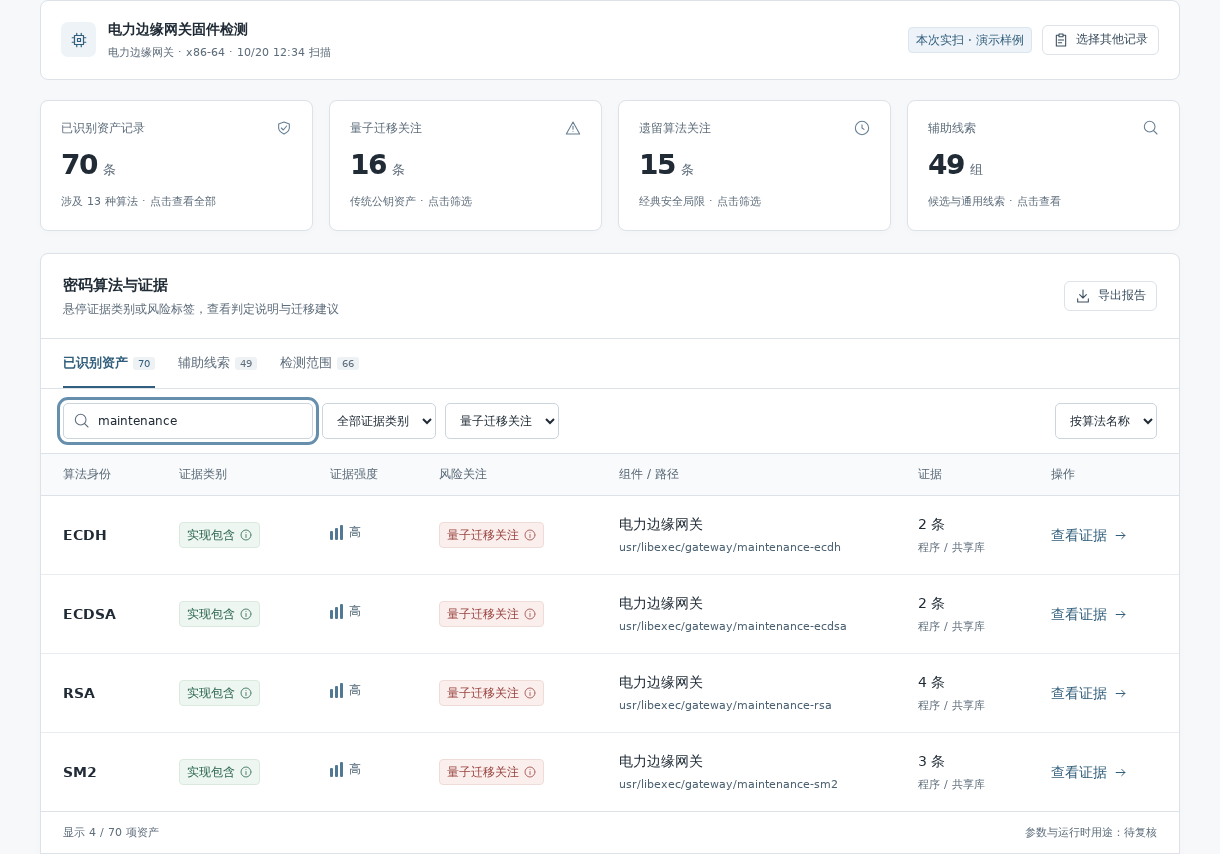
\includegraphics[width=\linewidth]{20-gateway-workbench-results.png}
\caption{网关的资产汇总及量子迁移关注筛选结果，列表展示部分公钥算法组件。}
\label{fig:gateway-workbench-results}
\end{figure}

结果另有 49 组辅助线索，单独保留候选名称与原始依据，不计入已识别资产。“量子迁移关注”用于提示传统公钥机制的替换评估，“遗留算法关注”用于提示 DES、RC4、MD5 和 SHA-1 的经典安全局限，其他资产仍需核对参数及用途。新增程序中的固定密钥只用于实验，不作为部署配置建议。静态结果没有证明全部算法均被原网关业务实际使用。

组件树包含外层镜像及 65 个提取文件，共 66 个条目。图~\ref{fig:gateway-workbench-components} 展示其中的镜像和密码组件，支持由算法回到文件位置。镜像摘要、内部路径和组件摘要在交付清单、独立提取结果及扫描报告中一致。该层级来自包含与提取关系，不表示组件调用或业务依赖。

\begin{figure}[H]\centering
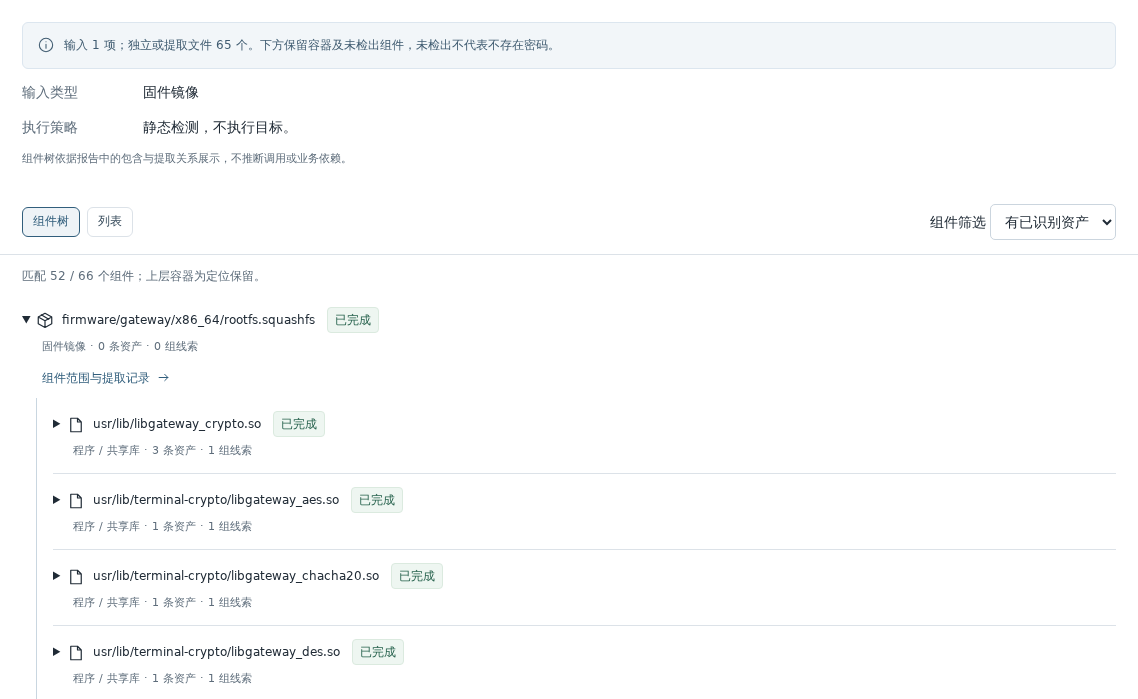
\includegraphics[width=\linewidth]{21-gateway-workbench-components.png}
\caption{网关镜像与内部密码组件的定位关系，视图展示组件树的一部分。}
\label{fig:gateway-workbench-components}
\end{figure}

以原密码库中的 AES 为例，证据详情同时列出数据表和参考函数匹配依据，记录参考函数 \texttt{aes\_encrypt}、文件偏移 \texttt{0x34e0}、匹配长度及引用数据约束。图~\ref{fig:gateway-workbench-evidence} 展示该条参考匹配。新增签名和密钥协商组件则可查看相应函数定义证据及文件位置，按其实际证据类别复核，不将符号定义识别解释为去符号算法恢复。

% 参考函数记录对应静态文件内容，不代表运行时调用或完整算法等价证明。
\begin{figure}[H]\centering
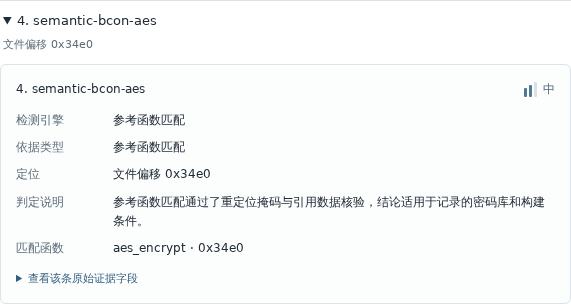
\includegraphics[width=.88\linewidth]{22-gateway-workbench-evidence.png}
\caption{AES 参考函数匹配的证据详情，包含函数名称、文件偏移和原始字段入口。}
\label{fig:gateway-workbench-evidence}
\end{figure}

\subsection{报告一致性与界面验证结果}

汇总 JSON、原始证据 JSON、CSV 表格和 Markdown 文本报告均保留 70 条已识别资产及 49 组辅助线索，任务标识与原始扫描一致。原始证据报告同时包含镜像与组件记录，可在页面之外核对输入身份及证据位置。搜索或风险筛选仅影响当前列表，导出文件仍保留完整任务结果。图~\ref{fig:gateway-workbench-report} 为同一任务的中文报告预览。

\begin{figure}[H]\centering
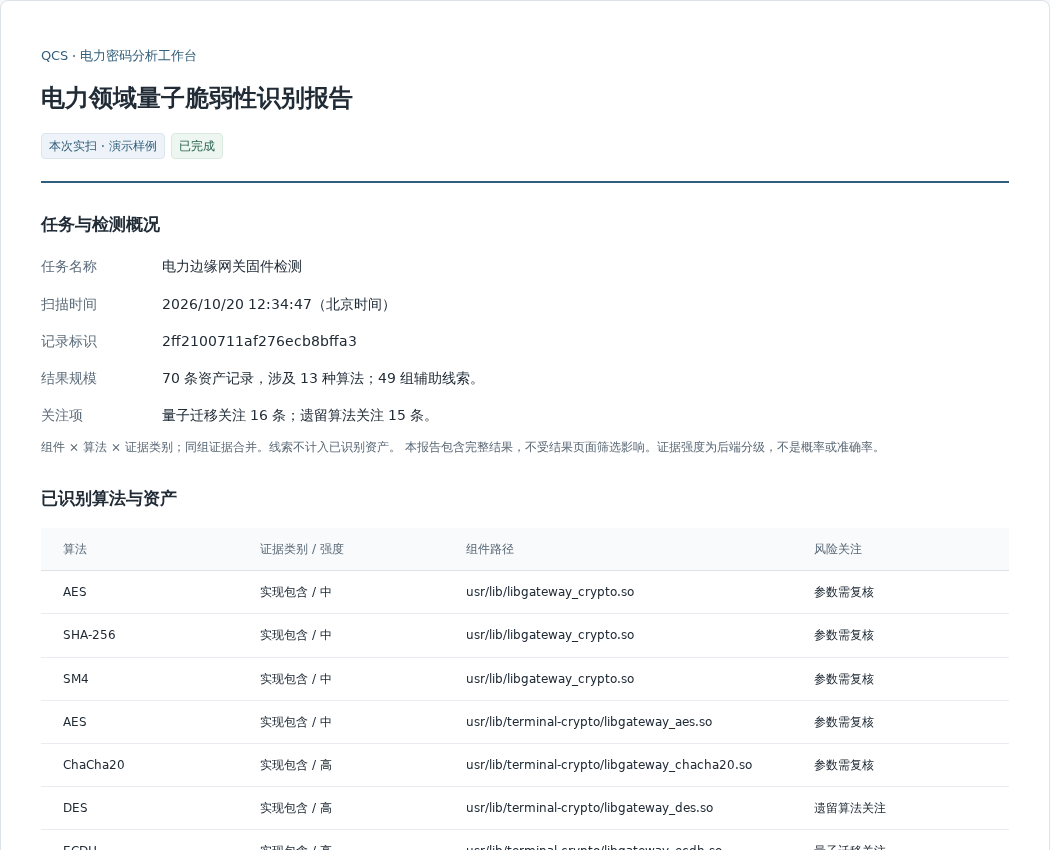
\includegraphics[width=\linewidth]{23-gateway-workbench-report.png}
\caption{网关任务的中文报告预览，汇总数值与页面及下载文件一致。}
\label{fig:gateway-workbench-report}
\end{figure}

中文报告经浏览器打印生成 32 页 A4 文档，包含资产清单、证据摘要、辅助线索与检测边界。Chromium 145 中的任务创建、结果检索、风险筛选、证据展开、组件定位及四种格式下载均正常完成，刷新后仍可读取任务结果。无匹配搜索显示空结果提示，在 1280 和 1440 像素宽度下均未出现整体横向溢出，交互过程中未发现未捕获的脚本异常。另从上传入口提交同版本镜像，核对接收摘要、组件数和算法种类，以确认新增镜像能够用于用户上传演示。

\section{结果讨论与适用范围}

已知实现集合的 97.19\% 召回率与源码参考补充后的 96.23\% 召回率分别对应不同材料和评分范围，不能合并为总体性能。前者的样本参与过规则与参考库修订，后者新增参考全部取自被测集合，均主要反映已知版本覆盖。作为对照背景，早期检测版本在 2855 份历史输入上的 TP/FP/FN 为 684/6/771，召回率为 47.01\%，显示不同实现与构建条件下仍存在明显缺口。由于材料、版本和评分范围不一致，该历史成绩仅用于说明外部有效性的限制，不与主体实验计算提升幅度。

受限语义后端在 18 组指令片段检查和 208 组数值对照中通过局部核查，但三批共 3339 份历史输入在接入前后的文件级算法预测没有变化，直接新增标签为零。因而，位宽及输入依赖约束具有局部结构检查依据，其对整体召回率的贡献尚未获得该对照支持。参考匹配、运算分析及语义后端的作用需要通过各自的消融结果评价，不能由综合成绩反推某一通道的独立增益。

错例同时反映出算法身份与分析完成度的区别。共享数学操作可能触发错误的协议标签，缺少实现主体或必要上下文则可能导致漏报；参考标签被识别后，受预算限制的结构分析仍可能部分完成。算法名称、证据位置、参数和处理状态应分别解释，才能避免以单个标签替代对完整实现及其用途的判断。

五类终端和网关均采用自制文件系统镜像，密码实现来源明确，部分与参考库共享来源，结果支持受控软件范围内的提取、识别和复核流程。真实厂商交付物、实体设备运行及后量子协议替换未在该应用实验中验证。界面风险提示用于引导参数与用途核查，尚不能作为网关整体抗量子安全结论。GraphRAG 和本地大模型仍处于方案设计阶段，本章不对其关联分析效果或运行开销作实测结论。

\section{本章小结}

已知实现覆盖实验在 1071 份输入、747 个正标签上取得 726/0/21 的 TP/FP/FN，召回率为 97.19\%。源码参考库消融在固定代码和材料条件下，将召回率由 70.75\% 提高到 96.23\%，增加 81 个正确标签，误报数量不变。分组与错例分析表明，已审核参考记录能够改善相应版本的覆盖，共享结构、上下文缺失及标注边界仍影响具体判断。

固件镜像实验完成五类终端共 10 份镜像的提取，恢复 650 个文件，其中 540 个二进制文件的 TP/FP/FN 为 657/1/45，召回率为 93.59\%，精确率为 99.85\%。网关前端应用实验形成 70 条资产记录，涉及十三种算法，并保持组件来源、证据位置及导出报告的一致性。上述结果支持受控软件材料的密码资产核查，未知实现覆盖与真实业务部署仍需进一步评价。
